\section{Bands, primary hard pins, and conditional data}\label{sec:pins}

Fix \(b>0\) with \(a=a(b)>0\).
The free limits from Section~\ref{sec:heights} must be transferred
to hard pins, and then to conditional laws at random guard data.
These are stronger statements than convergence of finitely many
unconditioned smears. We prove the transfer using the cable
exploration of \Bcite{an:path-poincare} and \Bcite{an:reach}, with
primary reference costs replacing bare Gaussian variances.
The loss of Gaussian tails under subdivision is handled by
polynomial damping and a separate truncation of large tilts.

\subsection{Geometry and the required limits}

Throughout this section a fixed geometry is a finite union of
bounded rectangular pieces with nondegenerate faces and widths.
Pieces in one component are joined along full interfaces, which
may be subdivided into segments. Point contacts do not identify
components, and opposite sectors are not joined only through a
vertex. Equivalently, we use the polygonal Lipschitz geometries
of \Bcite{an:geometry}, including the cut geometries there.
The nearest-neighbor primary lattice has mesh \(n^{-1}\).
Aligned boundaries may be rounded by a bounded number of lattice
steps, preserving the faces, corners, and positive-width passages.
All assertions also hold along sequences of such roundings.
A hard pin on a region means that every \emph{primary} height in
that region is zero; it does not pin the internal subdivision
vertices. Pin regions are aligned unions of positive-area boxes.

The ordinary unit-edge real Dirichlet form is the reference form.
On a component \(U\) with pin region \(p\), its limiting energy
space is
\[
 \mathcal H_{U,p}=\{v\in H^1(U):v=0\text{ almost everywhere on }p\},
 \qquad \mathcal E_U(v)=\int_U|\nabla v|^2.
\]
For an empty pin we take this space modulo constants when needed.
Free walls are understood in the variational, hence Neumann, sense.
The real form approximation, Poincare estimates, and energy
density statements in \Bcite{an:forms} apply to these ordinary
nearest-neighbor forms.

\begin{theorem}[Mixed height limits]\label{thm:mixed-limits}
For every fixed geometry above and every \(a(b)>0\), the massless
height law with primary hard pins has Gaussian Laplace and moment
limits for fixed bounded, piecewise continuous density smears.
On a component meeting a pin, the covariance is the inverse of
\[
                   a^{-1}\mathcal E_U
                   \quad\hbox{on }\mathcal H_{U,p}.
\]
On an unpinned component this assertion concerns mean-free smears.
Its fractional mean modulo \(2\pi\) is asymptotically uniform and
independent of the mean-free Gaussian field.

Adding a fixed finite-rank nonnegative quadratic penalty in box
averages gives the corresponding Gaussian law. If the penalty
controls every unpinned component constant, lattice translations
are summed and the limiting constants are integrated; the result
is an ordinary, unprojected Gaussian law. The assertions include
energy-approximable shifts and hold along every admissible primary
mesh sequence.
\end{theorem}

The second conclusion concerns the centered \emph{high law}
\(\mu_n\), obtained by adding
\(\norm{B_nh}^2/2\), where \(B_n\) is a fixed finite collection of
box averages controlling all component constants. Each defining
box lies wholly in one pre-pin component, so this high-law
penalty is a sum of component-local terms. For positively
separated box regions \(H,p\), initially without hard pins, put
\begin{equation}
 D_n(H,p)=\log
 \frac{\mu_n(h_H=0\mid h_p=0)}{\mu_n(h_H=0)},\qquad
 r_{H,n}(b^p)=
 \frac{\mu_n(h_H=0\mid h_p=b^p)}
      {\mu_n(h_H=0\mid h_p=0)}.
 \label{eq:pins-definitions}
\end{equation}
Regions lying in different components contribute independently.

We use the following precise meaning of convergence at random pin
data. Choose an increasing total list of smooth density probes
inside \(p\). A function of \(h_p\) has a Gaussian
\emph{finite-observation approximation} if, for every tolerance,
it can be approximated in probability by a function of a
sufficiently long fixed list of these probes, whose joint law and
function converge to the Gaussian counterparts. The probe list is
increased after the primary lattice limit. No pointwise continuum
trace, or uniform approximation at all microscopic pin values, is
asserted.

\begin{theorem}[Separated pin interaction and conditional laws]
\label{thm:pin-interaction}
Under the centered high law, \(D_n(H,p)\ge0\) converges to the
Gaussian pin interaction for precision
\[
                 a^{-1}\mathcal E_U(v)+\norm{Bv}^2.
\]
For every fixed finite list of density or box smears \(X\), the
conditional Laplace transforms and conditional weak laws given
\(h_p\) have the Gaussian finite-observation approximations just
defined. Moreover,
\[
 0<r_{H,n}\le1,\qquad
 \E_{\mu_n}r_{H,n}=e^{-D_n(H,p)},
\]
and \(r_{H,n}\) has the corresponding Gaussian approximation,
whose limit is strictly positive almost surely.
The convergence assertions persist when data are sampled under
a fixed finite linear exponential tilt, with \(D_n\) and
\(r_{H,n}\) retaining their centered definitions and the limiting
law sampled under the corresponding Gaussian tilt.
The displayed expectation identity concerns \(\mu_n\), not its
tilts. Conditional transforms for a tilted baseline also
converge, by taking ratios of the centered conditional transforms.
\end{theorem}

Both theorems are proved below. The Gaussian determinant and
localization facts used in the second theorem are
\Bcite{an:gaussian-localization}, applied to the ordinary real
nearest-neighbor form, not to the subdivided bare form.

\subsection{A confining band and uniform primary estimates}

It is enough initially to work in one fixed free component \(U\).
Choose a positive-width band \(K\) between a starting region and
a test region, with positive gaps on both sides. Partition \(K\)
into rectangles \(d\) of side comparable to \(\ell\) and bounded
aspect ratio. Write \(h_d\) for a primary probability average and
\(|d|\) for its scaled counting area. Define
\begin{equation}
 W_{\ell,\lambda}(h)=
 \exp\left\{-\frac{\lambda}{2}\sum_d|d|h_d^2\right\}.
 \label{eq:pins-band}
\end{equation}
Let \(\mathcal P_n\) be the sigma-finite free measure obtained by
normalizing one representative of each common-translation orbit
and summing \(h+2\pi m\), \(m\in\Z\). Changing the representative
only relabels this sum. The band law is
\[
 \dd\mathcal P_{n,W}=\widehat W\,\dd\mathcal P_n,\qquad
 \widehat W=W/\mathcal P_n(W).
\]
Its denominator is finite and positive. We always take limits in
the order
\begin{equation}
 n\longrightarrow\infty,\qquad
 \ell\downarrow0,\qquad
 \lambda\longrightarrow\infty.
 \label{eq:pins-limit-order}
\end{equation}
Subdivision size \(N\) is taken sufficiently large at each fixed
primary graph, or first through a fixed-graph limsup in the
uniform estimates below.

Before introducing pins, the free Gaussian limits on \(U\) follow
from Theorem~\ref{thm:free-limits} by the enclosing-rectangle
argument of \Bcite{an:forms}. Cut the enclosing rectangle into
the prescribed pieces. Smooth-gradient seam errors have
vanishing primary reference cost. Each partial observation has
the limiting variance upper bound \(a\) times its energy.
Subtracting the bounds for the other pieces from the saturated
enclosing observation gives saturation on each piece.
Energy density and the primary inverse-form approximation extend
this conclusion to the required smears. For a component phase
of nonzero integer total charge, precision monotonicity bounds
its characteristic function by the enclosing-rectangle one.
Theorem~\ref{thm:coefficient-gap}, also with mean-free sources,
therefore gives the independent uniform fractional mean on each
free component.

\begin{lemma}[Band density bounds]\label{lem:pins-band-density}
For every fixed \(\lambda>0\), \(q\ge0\), and \(1\le p<\infty\),
\begin{equation}
 \limsup_{\ell\downarrow0}\limsup_{n\to\infty}
 \mathcal P_n\bigl(\widehat W^p(1+|S|)^q\bigr)<\infty,
 \qquad S=(h,u),
 \label{eq:pins-density-moments}
\end{equation}
where \(u\) is the uniform primary probability on \(U\).
In the first two limits of \eqref{eq:pins-limit-order}, fixed
density smears under the band law converge with every fixed
moment to the Gaussian field of precision
\[
                 T_\lambda=-\Delta_U/a+\lambda1_K.
\]
For a smooth shift \(g\) vanishing near \(K\),
its weak Neumann Laplacian test has limiting variance
\(a\mathcal E_U(g)\), including its free-face terms.
Its limiting fourth moment is bounded uniformly for
\(\lambda\ge\lambda_0>0\).
\end{lemma}

\begin{proof}
At a fixed band partition, the free limits and the uniform
fractional mean make translation summation converge to integration
of the constant against \(\dd c/(2\pi)\). To justify unbounded
insertions, let \(\bar h_K=|K|^{-1}\sum_d|d|h_d\).
The band energy is at least \(\lambda|K|\bar h_K^2/2\), while
\(S-\bar h_K\) is a mean-free test of bounded primary reference
cost. Lemma~\ref{lem:reference-cost} supplies all its moments
and fixed linear exponential moments. Summing the Gaussian
translation tail gives uniform integrability for every fixed
polynomial insertion. This also proves convergence of the
normalizing constants and of the weighted moments at each fixed
partition.

After that limit, integrate the constant first. On the mean-free
Neumann field the remaining quadratic penalty is the squared
\(L^2(K)\) norm of its cell projection after subtracting its
\(K\)-average. Its covariance \(C_\ell\) satisfies
\(\sup_\ell\norm{C_\ell}_{\mathrm{HS}}<\infty\):
the square's inverse Neumann eigenvalues are square summable;
cutting a permitted domain into finitely many rectangles gives
the same bound by the compact energy inclusions of
\Bcite{an:forms}. If \(t_j\) are the eigenvalues of
\(\lambda C_\ell\), the logarithm of the determinant ratio in
the normalized \(p\)-th weight moment is
\[
 \frac12\sum_j\{p\log(1+t_j)-\log(1+pt_j)\}
 \le C_p\sum_jt_j^2.
\]
The constant integrals are bounded positive factors.
Poincare's inequality and control of the constant by the band
give, uniformly under cell refinement,
\[
 \norm v_{L^2(U)}^2\le C_\lambda
 \left(a^{-1}\mathcal E_U(v)+\lambda\sum_d|d|v_d^2\right).
\]
Thus every fixed moment of \(S\) under the continuum
\(p\)-weighted law is bounded. This proves
\eqref{eq:pins-density-moments} in its stated iterated-limsup
sense. It does not assert a lattice quadratic-exponential
moment.

Strong convergence of the cell projections in \(L^2(K)\),
weak energy compactness, and smooth recovery sequences give
convergence of the inverse forms to \(T_\lambda^{-1}\), exactly
as in \Bcite{an:band-density}. These prove the finite Gaussian
limits. If \(g\) vanishes near \(K\), then in the weak Neumann
sense \(T_\lambda(ag)=-\Delta_Ug\); hence its test variance is
\(a\mathcal E_U(g)\). Gaussian covariance decreases with
\(\lambda\), which proves the fourth-moment assertion.
\end{proof}

Metric-graph Gaussian sign clusters and their Markov exploration
are developed in \cite[Section~3 and Lemma~3.2]{Lupu2016}; the
integer-restricted Gaussian cable construction appears in
\cite[Section~7, Proposition~7.1]{AHPS2022}. For Bessel heights,
\cite[Section~2.2, Remark~1]{vEL} gives a cable construction
using conditioned differences of Poisson processes. Here we use
Gaussian cables on the finite series approximants and prove the
uniform primary-observation estimates needed to pass to Bessel
weights. On the \(N\)-subdivided lattice use the Gaussian chain
weights from Lemma~\ref{lem:comparisons}. Give each quadratic
bond its independent Brownian bridge conditional on endpoint
heights. A bond is open when its bridge does not hit zero.
Conditional on magnitudes and this open graph, nonzero
components have independent fair signs. Exploration reveals a
bridge only until its next vertex or its first zero. The
unobserved remainder starts at zero and has a shorter bridge
time, hence increased precision. Conditional on a completed
exploration, the unvisited law before band weighting is a
centered Gaussian lattice law with additional zero pins and
tightened outgoing segments. These are the finite-dimensional
bridge facts used in \Bcite{an:sign-disintegration}.
More explicitly, the remaining transition kernel at a stopped
segment is proportional to \(p_t(0,h_y)\), with \(t\) no larger
than its original time, regardless of the nonzero value from
which the revealed part began. That revealed value contributes
only to the exposed part of an observation and, after band
weighting, to its linear cross-term. For a centered unvisited
test, setting visited primary coordinates to zero is its zero
extension, not an assertion that their exposed values were zero.

Only primary heights contribute to smears or cluster masses.
A cluster carrying primary mass is counted once, for example by
its least primary vertex. A cluster of positive macroscopic
diameter contains a primary path with bounded successive steps.
Clusters confined to a single original edge have vanishing
scaled diameter.

For clarity, the uniform estimate behind this use of the cable
is elementary. With \(q=b/(2N)\), for \(|t|\le R\),
\begin{equation}
 \log\frac{\sum_{j\in\Z}q^{j^2}e^{2\pi tj}}
                {\sum_{j\in\Z}q^{j^2}}
       \le C_{b,R}t^2/N
       \qquad(N\hbox{ sufficiently large}).
 \label{eq:pins-chain-mgf}
\end{equation}
Group opposite \(j\)'s and use
\(\cosh(2\pi tj)-1\le C_Rt^2j^2e^{2\pi R|j|}\);
the resulting series is \(O_{b,R}(t^2/N)\).
Extending a unit-edge flow through a full chain therefore costs
at most a constant times its squared coefficient. Additional
internal zero pins or shorter cable segments only improve this
centered exponential comparison. In particular it is not the
bare series resistance that is used.

\begin{lemma}[Primary path anchoring]\label{lem:pins-path}
After exposure of a cluster of scaled diameter at least \(r>0\),
the centered posterior moments of every fixed primary density
smear are bounded in terms of its unit-edge reference cost,
uniformly in subdivision. The remaining full-component mean has
reference cost at most \(V_r\).
If \(\mathcal D\) consists of band cells touched by the exposed
path, and \(\ell<r/C\), the reference cost of
\(\sum_{d\in\mathcal D}|d|b_dh_d^U\) is at most
\begin{equation}
                 C\ell^2\sum_{d\in\mathcal D}|d|b_d^2.
 \label{eq:pins-local-path}
\end{equation}
Here averages retain the full primary cell denominator.
The same conclusions hold for exploration from an entire filled
starting region. A probability average in a cell reached by a
path from a fixed multiple of its diameter away has a uniformly
bounded posterior reference cost.
\end{lemma}

\begin{proof}
Extend variations on unvisited primary vertices by zero on the
visited primary set. Apply the ordinary unit-edge
path-Poincare argument of \Bcite{an:path-poincare}: in a
fixed-factor enlargement of a touched cell, stop the primary
path after it spans a comparable cell distance. One coordinate
spans a positive fraction of the lattice levels, giving anchored
rows or columns. One-dimensional telescoping on those rows,
followed by rectangle Poincare, bounds the cell's scaled
\(L^2\) norm by \(C\ell^2\) times its local unit-edge energy.
The enlargements have bounded overlap. Duality with flows gives
\eqref{eq:pins-local-path}. A macroscopic anchored rectangle and
global Poincare control the full-component mean.

At a free wall or a permitted junction, use the bounded union
of comparable rectangles within the same component. Their face
Poincare inequalities control differences of rectangle means.
The no-opposite-only convention ensures these rectangles are
joined through faces; one anchored rectangle anchors the union.
A filled starting region provides the initial zeros.
For a normalized cell average its squared \(L^2\) density is
\(O(\ell^{-2})\), canceling the local \(\ell^2\).

These are inequalities for the primary reference network.
Extend the optimizing flows through chains and use
\eqref{eq:pins-chain-mgf}, imposing the posterior constraints
and increased precisions by Lemma~\ref{lem:comparisons}.
One may insert the removed internal vertices at zero, ground
them, and tighten the first surviving segment; the resulting
centered quadratic law is precisely the unvisited posterior.
The flow identity involves only the unvisited test, since all
inserted and visited coordinates in this comparison are zero.
This transfers the inequalities to centered posterior moments,
uniformly in \(N\).
\end{proof}

\subsection{Polynomial damping and asymptotically fair signs}

Write the sigma-finite cable measure as
\(\nu_n(\dd\omega)\mathcal R_\omega(\dd\sigma)\), where \(\omega\)
is signless data and \(\mathcal R_\omega\) gives fair independent
cluster signs. For a primary smear \(f\), put
\[
 M_C(f)=\sum_{x\in C}|h_x|f_x,\qquad
 m_C=M_C(u),\qquad Q=\sum_Cm_C^2.
\]
All nonnegative calculations can first be made by Tonelli,
before finiteness of the sigma-finite integrals is known.
For a mean-free smear \(f\), let \(\mathcal R(f)\) denote its
minimum unit-edge squared flow cost.

\begin{lemma}[Bins, reinsertion, and polynomial tails]
\label{lem:pins-tails}
For \(t\ge1\) and every integer \(p\ge1\),
\begin{align}
 \nu_n(Q\le4t^2)&\le C(1+t),\notag\\
 \int_{Q\le4t^2}
       \left(\sum_CM_C(f)^2\right)^p\dd\nu_n
 &\le C_p(1+t)
 \left(t\left|\sum_xf_x\right|
       +\mathcal R(f-u\textstyle\sum_xf_x)^{1/2}\right)^{2p}.
 \label{eq:pins-bin}
\end{align}
After exposure of a cluster of diameter at least \(r\), the
complement squared-mass sum \(Q_U\) has conditional moments of
every fixed order bounded uniformly by constants depending on
that order and \(r\). Consequently, for every nonnegative
intrinsic completed-cluster cost \(I(C)\), and all sufficiently
large \(t=t(r)\),
\begin{equation}
 \int\sum_{\diam C\ge r}I(C)1_{\{m_C\le2t\}}\dd\nu_n
 \le
 2\int1_{\{Q\le8t^2\}}
       \sum_{\diam C\ge r}I(C)1_{\{m_C\le2t\}}\dd\nu_n.
 \label{eq:pins-reinsertion}
\end{equation}
For every \(j>0\) there is a sufficiently large \(M\) such that
\begin{equation}
 \mathcal P_n\left((1+|S|)^{-M}
                   1_{\{t^2<Q\le4t^2\}}\right)
       \le C_j(1+t)^{-j}.
 \label{eq:pins-damped-tail}
\end{equation}
All estimates are uniform in large subdivision and fine primary
mesh on the fixed geometry.
\end{lemma}

\begin{proof}
Given signless data, \(\E_\sigma S^2=Q\).
On \(Q\le4t^2\), Chebyshev gives high probability of
\(|S|\le Ct\). For \(Y=(h,f)\), the Rademacher fourth-moment
bound and Paley--Zygmund give a fixed positive probability of
\[
             |Y|\ge c\left(\sum_CM_C(f)^2\right)^{1/2}.
\]
Choose \(C\) so the two events intersect with a fixed positive
probability. On every translation orbit, \(|S|\le Ct\)
allows at most \(C'(1+t)\) translations. A mean-free \(Y\) is
translation invariant and has moments of every order bounded by
Lemma~\ref{lem:reference-cost}. This gives arbitrary polynomial
bin tails, and integration gives \eqref{eq:pins-bin}. For
nonzero total charge, use
\(Y=(h,f-u\sum f)+S\sum f\) on the same intersection.

After a macroscopic cluster is exposed, let \(S_U\) be the
complement signed mean. Lemma~\ref{lem:pins-path} gives every
conditional moment of \(S_U\), uniformly. Jensen in its remaining
fair signs yields
\[
 Q_U^p\le\E_\sigma|S_U|^{2p}.
\]
Thus \(\Prob(Q_U\le4t^2\mid\mathcal F_C)\ge1/2\) for
sufficiently large \(t\). If \(m_C\le2t\), this event implies
\(Q\le8t^2\). Multiply by \(I(C)1_{\{m_C\le2t\}}\), condition,
and sum by the least-primary-root disintegration. This proves
\eqref{eq:pins-reinsertion}, also for initially extended
nonnegative integrals.

For \eqref{eq:pins-damped-tail}, choose a small fixed diameter
threshold \(r\) and finitely many separated probability box
smears \(p_j\) so every cluster of diameter below \(r\) misses
one box. If small clusters contribute at least \(t^2/2\) to
\(Q\), assign each a missed box. Since
\(M_C(p_j-u)=-m_C\) there, one mean-free squared-mass sum is
at least \(ct^2\). Its polynomial bin tail, of an arbitrarily
high order, controls this part.

Otherwise the macroscopic clusters supply the majorant
\[
 1_{\{t^2<Q\le4t^2\}}
 \le\sum_{\diam C\ge r}
       \frac{2m_C^2}{t^2}1_{\{m_C\le2t\}}1_{\{Q>t^2\}}.
\]
Expose \(C\), and write \(S=\sigma_Cm_C+S_U\).
If \(m_C\ge t/2\), separate \(|S_U|\le m_C/2\)
from its complement. Polynomial damping handles the first event;
arbitrarily high conditional moments of \(S_U\) handle the
second. If \(m_C<t/2\), the condition \(Q>t^2\) forces
\(Q_U>3t^2/4\), again giving arbitrary polynomial decay.
Precisely, retain the intrinsic cost
\[
 I_t(C)=\frac{2m_C^2}{t^2}
              1_{\{\diam C\ge r,\ m_C\le2t\}}.
\]
After dropping the original upper-bin restriction, the
conditional expectation of
\((1+|\sigma_Cm_C+S_U|)^{-M}1_{\{m_C^2+Q_U>t^2\}}\)
is at most \(C_K(1+t)^{-K}\), uniformly on this intrinsic
cutoff, by the two cases just proved. This calculation is
under the unweighted base disintegration. Reinsertion gives
\[
 \int\sum_C I_t(C)\dd\nu_n
 \le2\int1_{\{Q\le8t^2\}}\sum_CI_t(C)\dd\nu_n
 \le32\,\nu_n(Q\le8t^2)=O(1+t).
\]
Choose \(K>j+1\). No weighted conditioning or count of
microscopic clusters enters this estimate.
\end{proof}

\begin{lemma}[Weighted cluster moments]\label{lem:pins-weighted}
At fixed \(\lambda\), all fixed moments of squared primary
cluster-mass sums and signlessly selected signed partial sums
are bounded in the first two limits of
\eqref{eq:pins-limit-order}. For a band cell \(d\), with
\(D_\ell^2=1+\log(1/\ell)\),
\begin{equation}
 \E_W\left(\sum_CM_C(d)^2\right)^p
       +\E_W|d_*|^{2p}
       \le C_{p,\lambda}D_\ell^{2p}+o_n(1).
 \label{eq:pins-cell-moments}
\end{equation}
Here \(d_*\) is any signed selection determined by signless data,
with nonnegative coefficients bounded by the full cell smear.
Fixed observation boxes have a fixed constant in place of
\(D_\ell\).
\end{lemma}

\begin{proof}
Let \(F\) be a squared-mass root or such a signed sum and let
\(A_t\) be a dyadic bin of \(Q\). Khintchine's inequality and
\eqref{eq:pins-bin} give
\(\mathcal P_n(|F|^{2p}1_{A_t})\le P_p(t)D^{2p}\),
where \(P_p\) is a polynomial and \(D\) the relevant reference
cost scale. Holder with exponents \(4,4,2\) gives
\begin{align*}
 \mathcal P_n(\widehat W|F|^p1_{A_t})
 &\le
 \mathcal P_n\bigl(\widehat W^4(1+|S|)^M\bigr)^{1/4}\\
 &\quad{}\times
 \mathcal P_n\bigl((1+|S|)^{-M}1_{A_t}\bigr)^{1/4}
 \mathcal P_n(|F|^{2p}1_{A_t})^{1/2}.
\end{align*}
The two polynomial weights cancel exactly. Use
Lemma~\ref{lem:pins-band-density} and choose the decay order in
\eqref{eq:pins-damped-tail} after \(p\), so that the dyadic sum
and its tail converge uniformly. The lowest bin is bounded
directly by \eqref{eq:pins-bin}.

The primary reference cost of \(h_d-S\) is
\(O(1+\log(1/\ell))\). On a containing rectangular patch,
sum the inverse Neumann cosine eigenvalues up to frequency
\(\ell^{-1}\); this costs \(O(\log(1/\ell))\).
Above that frequency Parseval and the squared density bound
\(O(\ell^{-2})\) give a bounded remainder. Component Poincare
compares the patch and component means. This proves
\eqref{eq:pins-cell-moments}. An auxiliary independent sign
sample has the same estimates, by exchanging the old and new
samples in the base measure.
\end{proof}

\begin{lemma}[Macroscopic sign resampling]\label{lem:pins-resampling}
At fixed \(r,\lambda>0\), replacing the signs of all clusters
of diameter at least \(r\) by independent fair signs changes
the band law by total variation tending to zero as
\(n\to\infty\) and then \(\ell\downarrow0\).
Clusters of diameter below \(r\) contribute vanishing fixed
moments to bounded density smears as \(r\downarrow0\) after
these limits. For nonnegative fixed density smears \(f,g\),
\begin{equation}
 \limsup_{\ell\downarrow0}\limsup_{n\to\infty}
 \E_W\sum_{\diam C\ge r}M_C(f)M_C(g)
       \le (f,T_\lambda^{-1}g).
 \label{eq:pins-cross}
\end{equation}
Every fixed moment of \(\sum_{\diam C\ge r}M_C(f)^2\)
has a limiting upper bound uniform for
\(\lambda\ge\lambda_0>0\).
\end{lemma}

\begin{proof}
On \(Q\le t^2\), expand the difference of the two quadratic
band energies in the original and new signs. Orthogonality of
Rademacher monomials bounds its squared base integral by
\[
 C\lambda^2\int1_{\{Q\le t^2\}}
 \sum_{\diam C\ge r}\sum_{C'\ne C}
       \left(\sum_d|d|M_C(d)M_{C'}(d)\right)^2\dd\nu_n.
\]
Expose \(C\), retain the intrinsic condition \(m_C\le t\),
and drop the complement bin restriction. Averaging the
complement signs turns the inner sum into the conditional
second moment of \(\sum_d|d|M_C(d)h_d^U\).
Lemma~\ref{lem:pins-path} bounds it by
\(C\ell^2\sum_d|d|M_C(d)^2\).
Reinsert a bin using \eqref{eq:pins-reinsertion}, and apply
\eqref{eq:pins-bin}. Thus
\[
 \mathcal P_n\left(1_{\{Q\le t^2\}}
       |\log W(\sigma')-\log W(\sigma)|^2\right)
 \le C_{\lambda,t,r}\ell^2D_\ell^2+o_n(1).
\]
The bin has finite base mass. The normalized densities have
uniform \(L^p\) bounds there. Split according to whether the
logarithmic difference exceeds a fixed \(\delta>0\), use
Holder on that exceptional set and
\(|e^x-e^y|\le(e^\delta-1)(e^x+e^y)\) on its complement.
Then let \(\delta\downarrow0\). Lemma~\ref{lem:pins-weighted}
removes the bin cutoff, including against observables with the
stated high moments.
For this last step, use the enlarged base space carrying the
old and new independent macroscopic sign samples, with the
small-cluster signs shared. Swapping the two samples preserves
the base measure and the signless variable \(Q\). Thus the old
and new normalized densities have identical \(Q\)-tails, and
for every fixed \(p\),
\[
 \int_{\{Q>T\}}|\widehat W(\sigma)-\widehat W(\sigma')|
 \le2T^{-p}\E_WQ^p.
\]
The right side is uniformly small in the first two limits.
For auxiliary-sign observables the unweighted bin moment
estimate is unchanged. For each density use its own component
mean in both damping factors; swapping the samples gives the
bound for the other density. Hence the weighted Holder
estimate controls those observables under either density.

Partition \(U\) into \(r\)-cells. A cluster of diameter below
\(r\) meets only boundedly many neighboring cells. For a bounded
density, Cauchy--Schwarz and \eqref{eq:pins-bin} bound its signed
second moment on a fixed bin by
\(C_t r^2(1+\log(1/r))\). Higher fixed moments are bounded
there. Interpolation, followed by the weighted tail transfer,
gives their vanishing.

Resample first at a threshold below \(r\), remove the smaller
clusters, and use Lemma~\ref{lem:pins-band-density}. Fair-sign
second moments are the cluster cross sums; nonnegative smears
make their summands nonnegative. This proves
\eqref{eq:pins-cross}. Jensen in the fair signs similarly
bounds the \(p\)-th moment of a squared-mass sum by the
Gaussian \(2p\)-th smear moment. The latter is uniformly
bounded for \(\lambda\ge\lambda_0\), since the Gaussian
covariance decreases with \(\lambda\).
\end{proof}

\subsection{Tilt errors and vanishing reach}

For an exploration under the band law, write
\(h_d=d_*+h_d^U\). Relative to the centered posterior with
the restricted band form, its remaining linear tilt is
\[
                  L=-\lambda\sum_d|d|d_*h_d^U.
\]
Lemma~\ref{lem:pins-path} bounds its reference cost by
\(\epsilon^2=C_0\lambda^2\ell^2\sum_d|d|d_*^2\).
For a single macroscopic cluster \(C\), define
\(\epsilon_C^2=C_0\lambda^2\ell^2\sum_d|d|M_C(d)^2\)
and \(E_2=\sum_{\diam C\ge r}\epsilon_C^2\).
Weighted Jensen and \eqref{eq:pins-cell-moments} give, for
every fixed \(p,\lambda,r\),
\begin{equation}
       \E_W\epsilon^{2p}+\E_WE_2^p
       \le C_{p,\lambda,r}\ell^{2p}D_\ell^{2p}+o_n(1).
 \label{eq:pins-tilt-moments}
\end{equation}

If \(\epsilon\le1\), the centered posterior \(\mu\) satisfies
\[
 1\le\mu(e^L),\qquad
 \mu(e^{2L})\le e^{C\epsilon^2},\qquad
 \mu((e^L-1)^2)\le C'\epsilon^2
\]
by \eqref{eq:pins-chain-mgf} and precision comparison.
Cauchy--Schwarz with fixed-cost fourth moments shows that
tilting changes means and second moments of fixed unexposed
smears by \(O(\epsilon)\). For an inversion-symmetric event
\(E\), symmetry also gives the relative estimate
\begin{equation}
       \mu_L(E)\ge e^{-C\epsilon^2}\mu(E).
 \label{eq:pins-relative-tilt}
\end{equation}
Indeed \(\mu(e^L\mid E)=\mu(\cosh L\mid E)\ge1\).
This estimate does not depend on the size of \(\mu(E)\).

Large tilts are truncated rather than estimated by a Gaussian
tail. Here is the exact summation needed for the size-biased
exploration. For comparison boxes \(B,i\), put
\[
 Q_B=\sum_{\diam C\ge r}M_C(B)^2,\qquad
 Q_i=\sum_{\diam C\ge r}M_C(i)^2.
\]
Since the number of clusters with \(\epsilon_C>1\) is at most
\(E_2\), pointwise
\begin{equation}
 \sum_{\diam C\ge r}M_C(B)1_{\{\epsilon_C>1\}}
       (1+h_i^2+M_C(i)^2)
 \le\sqrt{Q_BE_2}\,(1+h_i^2+Q_i).
 \label{eq:pins-bad-tilts}
\end{equation}
Its expectation vanishes by Holder, the actual band moments,
and \eqref{eq:pins-tilt-moments}. This controls the actual
unvisited contribution because
\(|h_i^U|\le|h_i|+M_C(i)\) after one-cluster exposure.
Centered comparison terms have the fixed-cost moment bounds.
For good tilts, Cauchy--Schwarz gives
\[
 \sum_C M_C(B)\epsilon_C(1+\epsilon_C)(1+M_C(i))
 \le\sqrt{Q_B}(1+\sqrt{Q_i})(\sqrt{E_2}+E_2),
\]
whose expectation also vanishes. For exterior exploration,
actual band moments and the vanishing moments of \(\epsilon\)
control the discarded event \(\epsilon>1\) directly.
These estimates use no quadratic-exponential moment of a
Bessel height and no subdivision-dependent bare variance.

We also need the size-bias inequality
\begin{equation}
                   \E[X^2|Y|]\ge\E X^2\,\E|Y|
 \label{eq:pins-size-bias}
\end{equation}
for real linear tests in a proper centered law with band
precision. On each subdivided Gaussian lattice it follows
from the minimal characteristic logarithmic Hessian:
for \(\phi(t)=\E\cos(tY)>0\),
\[
 \E[X^2\cos(tY)]\le\E X^2\,\phi(t).
\]
Subtract the identity at zero and integrate against
\(2\,\dd t/(\pi t^2)\), using
\(|y|=(2/\pi)\int_0^\infty(1-\cos ty)t^{-2}\dd t\).
Tonelli proves the inequality, and the fixed-graph moment
limit transfers it to primary heights. This is the
size-bias part of \Bcite{an:tilt}.

\begin{figure}[tbp]
\centering
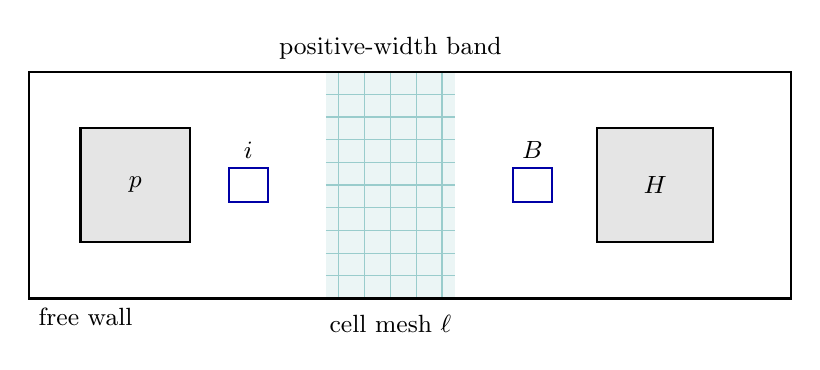
\begin{tikzpicture}[x=.82cm,y=.72cm,font=\small]
 \fill[teal!8] (4.6,0) rectangle (6.6,4);
 \draw[teal!40,step=.4] (4.6,0) grid (6.6,4);
 \draw[thick] (0,0) rectangle (11.8,4);
 \filldraw[fill=black!10,draw=black,thick] (.8,1) rectangle (2.5,3);
 \filldraw[fill=black!10,draw=black,thick] (8.8,1) rectangle (10.6,3);
 \draw[blue!65!black,thick] (3.1,1.7) rectangle (3.7,2.3);
 \draw[blue!65!black,thick] (7.5,1.7) rectangle (8.1,2.3);
 \node at (1.65,2) {$p$};
 \node at (9.7,2) {$H$};
 \node[above] at (5.6,4.05) {positive-width band};
 \node[above] at (3.4,2.3) {$i$};
 \node[above] at (7.8,2.3) {$B$};
 \node[below] at (5.6,-.12) {cell mesh $\ell$};
 \node[below right] at (0,0) {free wall};
\end{tikzpicture}
\caption{The band separates two positive-area pin regions.
The test boxes lie away from the band. Its cell mesh \(\ell\)
is refined while the physical band width stays fixed; the
band strength is increased only afterwards. Hard pins constrain
all primary height vertices in their regions.}
\label{fig:band}
\end{figure}


\begin{proposition}[Vanishing reach]\label{prop:pins-reach}
Under the band law, the probability that an exploration
starting in a fixed positive-area region on one side of a separating
positive-width band reaches a fixed closed region on the
other side tends to zero in \eqref{eq:pins-limit-order}.
The assertion includes exploration from a filled exterior
or from a primary hard-pin region before imposing its pin.
\end{proposition}

\begin{proof}
Choose finite small-cell coverings \(i\) on the starting
side and \(B\) on the target side, away from the band and
with positive clearances. Enlarge overlapping cells slightly
so every crossing path meets both coverings after rounding;
see Figure~\ref{fig:band}.
Concretely, first choose two separator strips, clipped to
the free component, with a fixed clearance \(\eta>0\) from
the band and the filled starting and target regions.
Then cover them by cells of radius \(\delta\ll\eta\).
A reaching path contains, in a fixed-factor enlargement
of the touched cell, a segment spanning \(c\delta\).
The path-Poincare constant on this rescaled patch depends
only on the fixed finite face and corner geometry, not on
\(\delta\); at a wall use the adjacent face-connected
rectangular pieces of that same component.
The primary path bound gives a uniform upper bound \(C_0\)
for the centered remaining average in a reached cell.
A logarithmic trial supported in a fixed ball away from
the band gives continuum prior variance at least
\(c\,a\log(1/\delta)-C\) for a cell of radius \(\delta\).
Cut the trial off at a radius \(\rho<\eta/4\) fixed before
\(\delta\). It pays no band mass. At a free wall or corner
restrict it to the component; this is an admissible Neumann
energy function. Its cell average is bounded below by
\(c\log(\rho/\delta)-C\), and its energy is at most
\(C\log(\rho/\delta)+C\), uniformly over the bounded cell
shapes. Thus shrinking the cells increases the prior lower
bound without increasing the path-anchoring constant.
Choose the covering cells so small that the prior variance
exceeds \(C_0+2c_0\), for some \(c_0>0\), uniformly in
\(\lambda\). At each fixed \(\lambda\), band convergence
gives the strict gap \(c_0\) on fine meshes.

For exterior exploration write \(h_B=e_B+u_B\), exposed
plus unexposed. The centered posterior is obtained by
zero-pinning visited vertices and increasing cable
precision. Thus its variance for \(u_B\) is at most
the full prior variance \(v_B\), and at most \(v_B-c_0\)
on a visit to \(B\). Restoring the tilt changes the
averaged second moment and cross term by \(o(1)\), by
the good- and bad-tilt estimates above. The identity
\(\E_Wh_B^2=v_B\) therefore gives
\(c_0\Prob_W(B\text{ reached})\le\E_We_B^2+o(1)\).
All contributing clusters are macroscopic, with a
threshold fixed by the separation from the starting set.
Sign resampling, with that same signless selection, yields
\begin{equation}
 c_0\Prob_W(B\text{ reached})
 \le\E_W\sum_{C\text{ meeting the starting set}}M_C(B)^2+o(1).
 \label{eq:pins-exterior-deficit}
\end{equation}

For the second deficit, bias the prior by \(|h_x|\),
where \(x\in B\), and expose only its cluster.
The pre-exposure second moment at \(i\) is at least
\(v_i\) by \eqref{eq:pins-size-bias}. The bias is measurable
at completed exploration, so cancels from the conditional
complement law. Its centered remaining variance is at
most \(v_i\), and at most \(v_i-c_0\) when the cluster
visits \(i\). Multiply the total second-moment comparison
by \(\E|h_x|\) and the primary averaging weight of \(x\),
then sum over \(x\in B\). This produces precisely the
weight \(M_C(B)\), not a count of microscopic clusters.
Only clusters reaching the band or \(i\) cause a
nonzero tilt or exposed term; the separating gaps make
all of them macroscopic. The estimates preceding the
proposition give
\begin{equation}
 c_0\E_W\sum_{C:C\cap i\ne\varnothing}M_C(B)
 \le\E_W\sum_C M_C(B)M_C(i)^2+o(1).
 \label{eq:pins-biased-deficit}
\end{equation}
Points with \(\E|h_x|=0\) contribute zero.

As \(\lambda\to\infty\), the inverse forms
\(T_\lambda^{-1}\) decrease to the inverse with every
energy function zero on \(K\). Weak energy compactness
and recovery by such functions prove this statement
directly. The hard band separates the sides, so its
cross covariance is zero. Equation~\eqref{eq:pins-cross}
therefore makes
\(\E\sum_CM_C(B)M_C(i)\) vanish in the prescribed order.
Truncate first at \(\max_CM_C(i)\le M\); on this event
the right side of \eqref{eq:pins-biased-deficit} is at
most \(M\) times that cross sum. Its remaining tail
vanishes uniformly as \(M\to\infty\), since
\[
             \sum_CM_C(B)M_C(i)^2\le\sqrt{Q_B}\,Q_i
\]
and Lemma~\ref{lem:pins-resampling} supplies arbitrarily
high moments uniform toward large \(\lambda\).
Consequently the first-mass sum on the left of
\eqref{eq:pins-biased-deficit} vanishes.
Every starting-set cluster meeting \(B\) visits one
of the finitely many cells \(i\). Truncate
\(\max_CM_C(B)\) in \eqref{eq:pins-exterior-deficit}
and use these first-mass bounds; its tail is controlled
by the moments of \(Q_B\). This proves vanishing reach.

All exploration calculations were on finite subdivided
Gaussian graphs. Their primary bounds are uniform in
large \(N\), or are passed first at a fixed primary
graph. Thus no continuum-time cable realization of the
limiting Bessel law is needed.
\end{proof}

\subsection{Mixed limits and relative hard-pin comparison}

\begin{proof}[Proof of Theorem~\ref{thm:mixed-limits}]
On a component meeting \(p\), start with a smooth shift
\(g\) vanishing near the entire pin but allowed to meet
the free walls. Choose a separating band between \(p\)
and its support, with fixed gaps. The band may be a
union of strips clipped to the component. Use the
ordinary mixed-domain geometry from \Bcite{an:mixed-scaling};
Lemma~\ref{lem:pins-path} already verifies its reference
inequalities at faces and junctions.

For the weak Neumann Laplacian test of \(g\), the band
variance is \(a\mathcal E_U(g)\).
Explore from every primary vertex of \(p\).
On success, the exposed test is zero and the centered
posterior has at least the desired primary pin, possibly
further zero pins, tighter chains, and restricted band
precision. Its variance is therefore at most that under
the desired massless hard-\(p\) law.
The tilt errors vanish as above. On failure the actual
second moment is bounded by its fourth-moment root
times the square root of the failure probability.
Lemma~\ref{lem:pins-band-density} bounds that fourth
moment uniformly after the first two limits and toward
large \(\lambda\). Proposition~\ref{prop:pins-reach}
therefore gives
\[
 \liminf_{n\to\infty}\Var_p(h,A g_n)
                  \ge a\mathcal E_U(g).
\]
Run the argument on an arbitrary primary subsequence.
The free variance upper bound gives the opposite
limsup. The free logarithmic transform upper bound
and the centered-variance lower bound under real tilt
then give the matching Gaussian Laplace limit.

Weak free-face terms may first be approximated by
bounded density smears in primary reference cost,
preserving their gap from \(p\) and the band.
The real mixed inverse-form approximation and density
of smooth shifts vanishing near \(p\), from
\Bcite{an:forms}, extend the result to all asserted
tests. Lemma~\ref{lem:reference-cost} controls the
errors independently of subdivision. It supplies
uniform integrability for every fixed linear
exponential and polynomial insertion.

Unpinned components were handled before
Lemma~\ref{lem:pins-band-density}. Finally integrate
a fixed finite-rank quadratic penalty against these
massless limits. On pinned components the preceding
moment bounds suffice. On unpinned components sum
translations and use the independent uniform
fractional mean, with the confining penalty controlling
the constants exactly as in the band-density proof.
This proves the theorem, including its limit order
and its statements for rounded geometry sequences.
\end{proof}

We now prove convergence of the interaction in
\eqref{eq:pins-definitions}; this is where a relative,
rather than absolute, estimate is essential.
Write \(U\) for the original finite box-average
penalty and \(W\) for a separating band penalty.
Let \(Z_{M,Q}\) be the partition sum with penalty
\(M\) and primary hard pin \(Q\). Cancellation gives
\begin{align}
 D_U-D_W
 &=\log\frac{Z_{U,H\cup p}}{Z_{W,H\cup p}}
   +\log\frac{Z_{U,\varnothing}}{Z_{W,\varnothing}}
   -\log\frac{Z_{U,H}}{Z_{W,H}}
   -\log\frac{Z_{U,p}}{Z_{W,p}}.
 \label{eq:pins-four-ratios}
\end{align}
Each ratio changes only a fixed finite-rank confining
penalty on one fixed massless pinned or unpinned
domain. Its common normalization cancels, so
Theorem~\ref{thm:mixed-limits} gives its Gaussian
limit at each fixed band partition and strength.
The real Gaussian determinant theorem
\Bcite{an:gaussian-localization} identifies the
corresponding interaction difference.

Under the unpinned band law, explore all clusters
meeting \(p\). On the event \(\mathcal S\) that
\(H\) is untouched, the centered posterior is
obtained from the band law conditioned on \(h_p=0\)
by further primary or internal zero pins and
increased precision. Its probability of \(h_H=0\)
is at least \(\mu_W(h_H=0\mid h_p=0)\).
For \(\epsilon\le\delta\le1\), the actual tilted
posterior therefore satisfies
\[
 \mu_W(h_H=0\mid\mathcal F)
 \ge e^{-C\delta^2}\mu_W(h_H=0\mid h_p=0).
\]
Averaging gives the relative estimate
\begin{equation}
 e^{-D_W}\ge e^{-C\delta^2}
                 \Prob_W(\mathcal S\cap\{\epsilon\le\delta\}).
 \label{eq:pins-relative-pin}
\end{equation}
It remains valid however small the two pin
probabilities are. By precision monotonicity
\(D_W\ge0\). First the tilt vanishes at fixed
\(\lambda\), then reach vanishes as \(\lambda\)
increases. Sending \(\delta\downarrow0\) proves
\(D_W\to0\) in \eqref{eq:pins-limit-order}.

The same vanishing holds for the real Gaussian
interaction \(D_W^{\mathrm g}\). One may use the
real-Gaussian proof of \Bcite{an:relative-pin-bound}:
replace pin probabilities by joint densities at
zero, use the same centered precision comparison,
and average small-box pin probabilities before
dividing by their volumes and applying Fatou.
The ordinary Gaussian localization theorem passes
the separated-pin determinants to the continuum.
Thus both band interactions vanish. Equation
\eqref{eq:pins-four-ratios} proves
\begin{equation}
                         D_n(H,p)\longrightarrow D^{\mathrm g}(H,p).
 \label{eq:pins-interaction-limit}
\end{equation}
No individual microscopic pin probability has been
assigned a positive continuum limit.

\subsection{Regression at typical pin data and restoration}

\begin{proof}[Proof of the remaining assertions of
Theorem~\ref{thm:pin-interaction}]
Let \(X_n\) be a fixed real smear,
\(m_n(b^p)=\E(X_n\mid h_p=b^p)\), and
\(v_{p,n}=\Var(X_n\mid h_p=0)\).
At prescribed primary data, the subdivided law is an
affine Gaussian lattice law with the same quadratic
part as at zero data. Lemma~\ref{lem:comparisons},
including an additional real tilt, and then its
fixed-graph limit give
\begin{equation}
       \Var(X_n\mid h_p=b^p;\text{ tilt }tX_n)\ge v_{p,n}.
 \label{eq:pins-conditional-variance}
\end{equation}

Choose the first \(J\) smooth density probes on \(p\),
and let \(L_n^{(J)}\) be their linear combination
with the limiting Gaussian regression coefficients.
Remove redundant directions or invert on their
Gram-matrix range. Conditional variance decomposition
gives the exact bound
\begin{align}
 \E|m_n-L_n^{(J)}|^2
 &=\E|X_n-L_n^{(J)}|^2
                   -\E\Var(X_n\mid h_p)\notag\\
 &\le \E|X_n-L_n^{(J)}|^2-v_{p,n}.
 \label{eq:pins-regression}
\end{align}
Theorem~\ref{thm:mixed-limits} identifies both limiting
variances. As \(J\to\infty\), totality of the pin
probes makes the right side tend to zero: in the
Gaussian energy space it is the squared difference
between the full pin projection and the \(J\)-probe
projection of the representer of \(X\).
Thus the conditional mean is approximated in \(L^2\)
by the finite Gaussian linear predictions.

Integrating \eqref{eq:pins-conditional-variance}
twice in \(t\) gives
\[
 Y_n:=\E(e^{X_n}\mid h_p)
             \ge\exp\{m_n+v_{p,n}/2\}.
\]
Both sides have limiting expectation \(e^{v/2}\),
where \(v\) is the full limiting variance.
For the right side, use \eqref{eq:pins-regression}
and uniform exponential integrability:
\(\E e^{q m_n}\le\E e^{qX_n}\) by Jensen for
every fixed real \(q\).
Their nonnegative difference tends to zero in
\(L^1\), proving the conditional Laplace assertion.
Apply the same argument to a countable dense set
of linear combinations of any fixed test list.
Subsequence extraction and conditional exponential
moment bounds give tightness and identify all
conditional finite-dimensional weak limits.
This also proves conditional convergence of fixed
smooth quadratic penalties.

For the pin ratio, precision comparison at prescribed
\(b^p\) shows that every normalized conditional
positive-penalty ratio is at most one and decreases
when the penalty is increased. Letting a full
coordinate pin on \(H\) tend to infinity yields
\(0<r_{H,n}\le1\). Its definition gives exactly
\(\E r_{H,n}=e^{-D_n}\).

Let \(Q_J\) be increasing finite smooth quadratic
penalties exhausting the pin on \(H\), and put
\[
 R_{J,n}(b^p)=
 \frac{\E(Q_J\mid h_p=b^p)}{\E(Q_J\mid h_p=0)}.
\]
Then \(r_{H,n}\le R_{J,n}\le1\).
For fixed \(J\), the conditional weak convergence
and the centered hard-\(p\) limit identify \(R_{J,n}\)
with its Gaussian counterpart. Moreover,
\begin{equation}
       \E(R_{J,n}-r_{H,n})=\E R_{J,n}-e^{-D_n}.
 \label{eq:pins-probe-gap}
\end{equation}
The interaction limit \eqref{eq:pins-interaction-limit}
and the finite-probe determinant approximation in
\Bcite{an:gaussian-localization} make the right side
tend to zero as \(J\to\infty\) after \(n\to\infty\).

More explicitly, let \(s_j\) be the singular values
of the cross projection between the Gaussian pin
spaces of \(p\) and \(H\). Positive separation gives
\(\sup_js_j<1\) and \(\sum_js_j^2<\infty\).
In canonical standard Gaussian pin coordinates
\(\xi_j\),
\[
 r_H^{\mathrm g}
 =\exp\left\{-\frac12\sum_j
           \frac{s_j^2}{1-s_j^2}\xi_j^2\right\}>0
 \quad\hbox{almost surely},\qquad
 \E r_H^{\mathrm g}=\prod_j\sqrt{1-s_j^2}=e^{-D^{\mathrm g}}.
\]
Finite probes exhaust these convergent expressions.
Markov's inequality in \eqref{eq:pins-probe-gap}
therefore proves the asserted finite-observation
approximation of the full ratio. In particular
\begin{equation}
 \lim_{\eta\downarrow0}\limsup_{n\to\infty}
                  \mu_n(r_{H,n}\le\eta)=0.
 \label{eq:pins-away-zero}
\end{equation}

Finally a fixed finite linear tilt has uniformly
bounded \(L^q\) density for every fixed finite \(q\):
its denominator is at least one, and the mixed
Laplace bounds control its numerator's moments.
Holder transfers the preceding convergence statements
to the tilted law. Here \(r_{H,n}\), \(D_n\), and the
conditional functions being sampled keep their centered
definitions; in particular we do not claim
\(\E_{\mu_{n,L}}r_{H,n}=e^{-D_n}\).
If a conditional transform under the tilted baseline is
needed, use
\[
 \E_{\mu_{n,L}}(e^X\mid h_p)
   =\frac{\E_{\mu_n}(e^{X+L}\mid h_p)}
          {\E_{\mu_n}(e^L\mid h_p)}.
\]
The denominator has a strictly positive Gaussian limit,
so the established joint conditional convergence applies.
This completes the theorem.
\end{proof}

\begin{lemma}[Restoration and two-way transfer]
\label{lem:restoration}
Let \(\mu_n\) be a cut centered high law and let
\(\nu_n\) restore bonds or positive forms supported
inside a core \(H\), separated from the guard \(p\).
Include both primary endpoints of every restored
bond, and the support of every restored form, in
the hard core pin. If \(Q_\Delta\) is the positive
restoration factor and
\[
 r_\Delta(b^p)=
 \frac{\E_{\mu_n}(Q_\Delta\mid h_p=b^p)}
      {\E_{\mu_n}(Q_\Delta\mid h_p=0)},
\]
then
\begin{equation}
 r_{H,n}\le r_\Delta\le1,\qquad
 \frac{\dd\nu_{n,p}}{\dd\mu_{n,p}}
   =\frac{r_\Delta}{\E_{\mu_n}r_\Delta},\qquad
 r_{H,n}\le\frac{\dd\nu_{n,p}}{\dd\mu_{n,p}}
                  \le e^{D_n(H,p)}.
 \label{eq:pins-restoration}
\end{equation}
Events concerning random guard data whose probabilities
tend to zero transfer in both directions between
the two topologies. This typical-data transfer also
holds when either law is sampled with a fixed finite
linear tilt. The displayed identities and inequalities
remain statements about the centered laws and their
centered-defined ratios.
\end{lemma}

\begin{proof}
For each restored edge \(e=(x,y)\), enlarge the cut
law by an independent normalized chain of increments
\(\xi_{e,1},\ldots,\xi_{e,N}\in2\pi\Z\) in height units, and put
\(J_e=\sum_k\xi_{e,k}\). Restoring the edge imposes
\(J_e=h_y-h_x\). Conditional on primary heights, its
factor is the chain-convolution probability
\(p_{b,N}((h_y-h_x)/(2\pi))\), tending to the Bessel
weight. Thus the primary factor need not itself be
quadratic. On the expanded lattice, matching is the
limit of the positive quadratic penalties
\(\exp[-t(J_e-h_y+h_x)^2/2]\).

Write \(Z_{b^p}\) and \(Z_0\) for the expanded cut
sums at the two guard data, and use a superscript
\(\Delta\) for restored matching and any further
restored positive forms. The guard fibers are affine
and centered copies of the same expanded lattice, and
\[
 r_\Delta(b^p)=
       \frac{Z_{b^p}^{\Delta}/Z_{b^p}}
            {Z_0^{\Delta}/Z_0}.
\]
Precision comparison gives \(r_\Delta\le1\);
adding the full primary \(H\)-pin can only decrease
this ratio. With both endpoints pinned, every new
chain matches \(J_e=0\). Its integrated factor is
the scalar \(p_{b,N}(0)>0\), independent of guard
data. Hence
\(Z_{b^p}^{\Delta+H}=\kappa_N Z_{b^p}^{H}\)
and \(Z_0^{\Delta+H}=\kappa_N Z_0^{H}\), with the
same \(\kappa_N\). The resulting normalized ratio is
exactly \(r_{H,n}\), proving its lower bound.
All independent-chain normalizers were identical in
these sums, and both they and \(\kappa_N\) cancel.
Internal chain variables therefore need not be pinned.
Take matching penalties to infinity and then the
fixed-primary-graph subdivision limit.

Bayes' formula gives the middle identity in
\eqref{eq:pins-restoration}. Its denominator lies
in \([e^{-D_n},1]\), proving the last two bounds.
The interaction has a finite limit, so the upper
density bound transfers \(\mu_{n,p}(A_n)\to0\)
to \(\nu_{n,p}(A_n)\to0\). Conversely, for \(\eta>0\),
\[
 \mu_{n,p}(A_n)
 \le\mu_{n,p}(r_{H,n}\le\eta)
                       +\eta^{-1}\nu_{n,p}(A_n).
\]
Use \eqref{eq:pins-away-zero}, sending \(\eta\downarrow0\)
after the lattice limit. Fixed linear tilts transfer
by Holder and the bounds for both positive and
negative fixed exponential moments. All these
statements concern the finite-observation sense at
typical data specified above.
\end{proof}
